\chapter{Testing}

%Detailed descriptions of every test case are definitely not what is required here. What is important is to show that you adopted a sensible strategy that was, in principle, capable of testing the system adequately even if you did not have the time to test the system fully.

%Have you tested your system on 'real users'? For example, if your system is supposed to solve a problem for a business, then it would be appropriate to present your approach to involve the users in the testing process and to record the results that you obtained. Depending on the level of detail, it is likely that you would put any detailed results in an appendix.

\section{Overall Approach to Testing}
Testing any complex hardware of software system is a critical process because if there are any major points of failure the whole system could cease to operate.  Time does not always permit this but at least some general testing of all systems should be carried out to highlight any obvious problems.
\section{Automated Testing}
Automated testing is a very good process to be using as the system being developed is tested and the results of these tests whether they be positive or if they highlight problems with the system all without the developer having to do anything after the initial setup of this testing process.
\\Due to the embedded nature of this project, automated testing is very limited.  As there is no simulator for an arduino microcontroller and all the various components that can be used in conjunction with one, no automated testing of this can be achieved without a far more complex hardware system which somehow can test other hardware configurations.  The only part of the system that can be automatically tested with any degree of reliability is to parse the software code and check is it is syntactically valid.
\section{System Tests}
These are written to test each individual part of the project.  This starts with testing if the code validates.  A compiler is used to validate this and a compiler is another program that checks if code will actually work, not necessarily for its intended purpose but just check that it does not have a major flaw that will stop the finished program from running at all and converts it into either a binary capable of being run as an executable program or into another language.  This compiled code is what will run on the hardware itself rather than through an interpreter which is another program that interprets what the code is trying to do and runs that.
\\The next stage of testing is to check that the software for each individual hardware interaction works as expected.  This includes checking that when the code tells a motor to turn in a specific direction that it actually turns as it is told to.  A motor is laid out on a workbench, hooked up to the microcontroller and told to turn.  If it does as expected then the test will be considered as passed, otherwise it will be considered as failed and debugging will be required before running the tests again.
\\Similar tests will be run on the sensors with then placed at set distance intervals from objects and tested to see if the recorded distance measured by the sensor is the same as the real world measurement specifies.
\begin{figure}[h]
\centering
        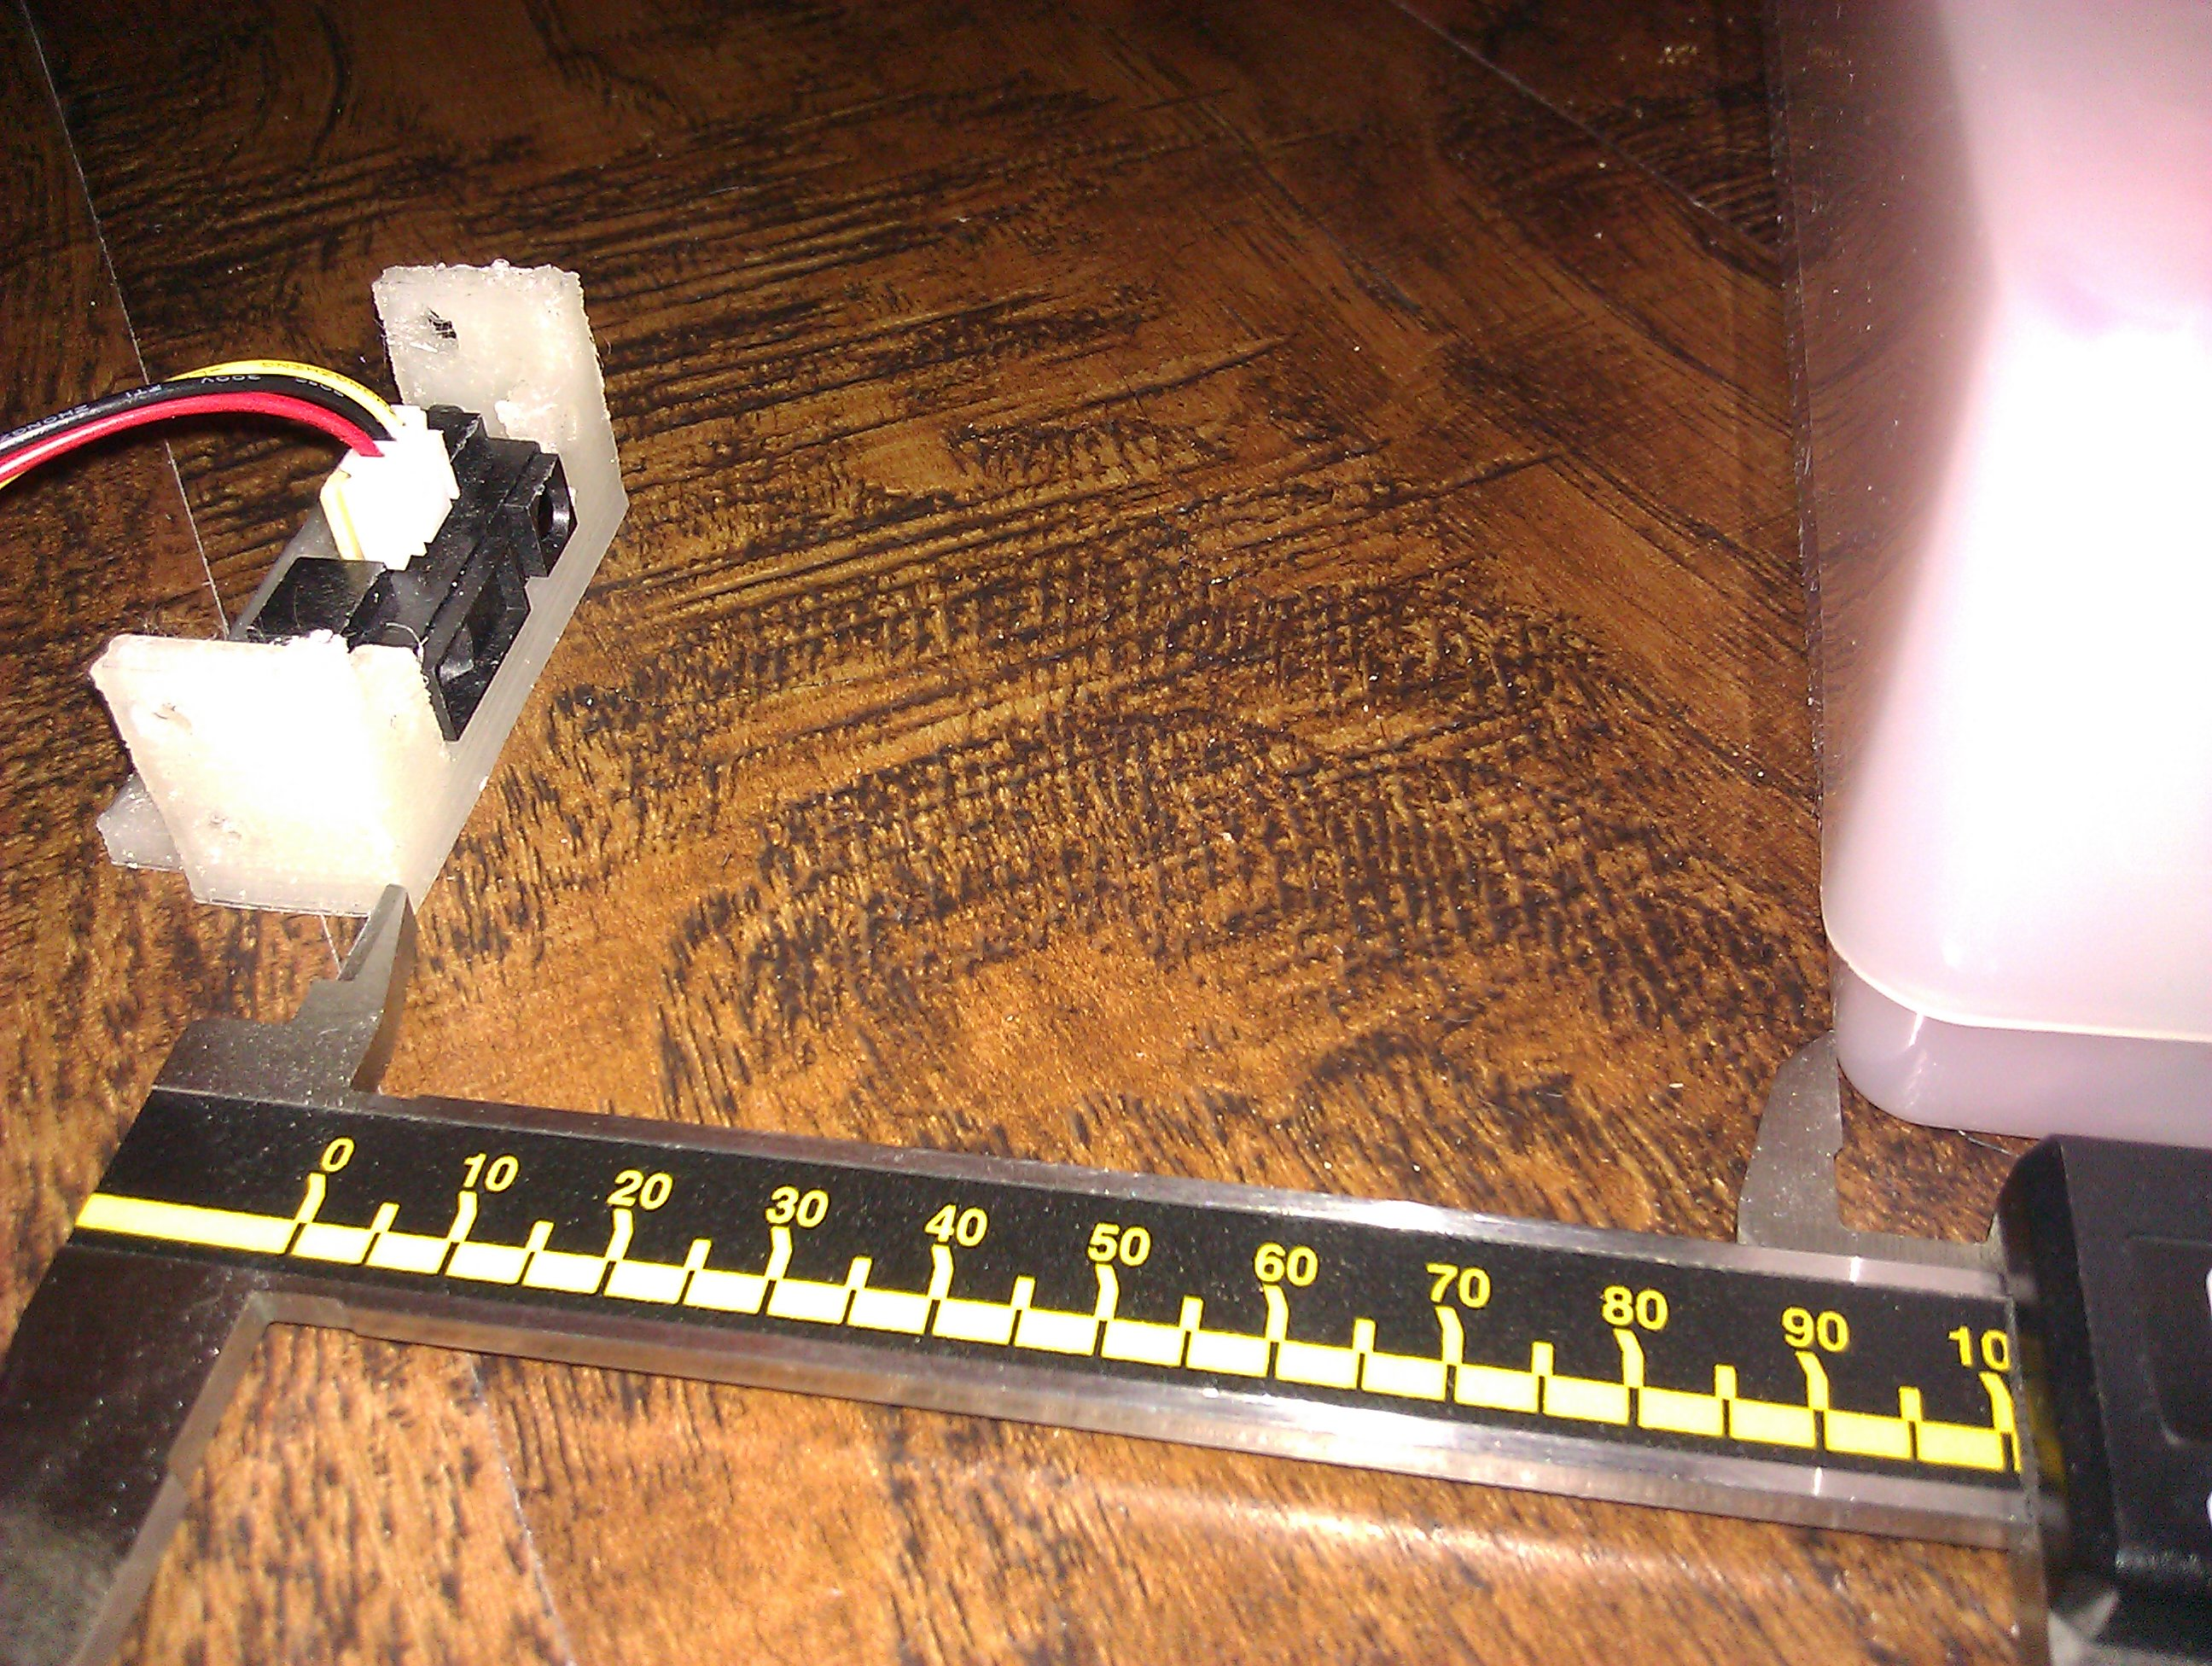
\includegraphics[width=4.0in] {Images/ir-measure-2.jpg}
        \caption{Infrared Distance Test}
        \label{Infrared Distance Test}
\end{figure}
\section{User Interface Testing}
The only user interface on the robot is a button to apply or cut off power to the system and an activity readout over a serial communication line.  This communication can either be over a USB (universal serial bus) cable or over some form of wireless serial such as bluetooth or the xbee module I am using.


